\documentclass[11pt]{beamer}
\usetheme{Luebeck}
%\usecolortheme{seahorse}
\useinnertheme{rectangles}
\useoutertheme{infolines}
\usepackage{xcolor}
\usepackage{natbib}
\usepackage[utf8]{inputenc}
\usepackage{tikz}
\usepackage{tabularx}
\usepackage{lipsum}
\usepackage{amsmath,graphicx,dsfont}
\usepackage{amssymb}
\usepackage{graphicx}
\usepackage{multirow}
\usetikzlibrary{shapes,backgrounds,arrows,automata,snakes,shadows,positioning, mindmap}
%\usepackage[citestyle=verbose]{biblatex}
%===================================
\newcommand\G{\mathcal{G}}
\newcommand\J{\mathcal{J}}
\newcommand{\Esp}{{\mathds{E}}}
\DeclareMathOperator*{\Cov}{\mathbb{C}\text{ov}}
% Notations tilde
\newcommand\Pt{\widetilde{P}}
\newcommand\pt{\widetilde{p}}
\newcommand\et{\widetilde{\mathds{E}}}
\newcommand\e{{\mathds{E}}}
\newcommand{\betabft}{{\widetilde{\betabf}}}
\newcommand{\Mbft}{{\widetilde{\Mbf}}}
\newcommand{\Sbft}{{\widetilde{\Sbf}}}
\newcommand\mt{\widetilde{m}}
\newcommand\St{\widetilde{S}}
\newcommand\mbt{\widetilde{\bf m}}
\newcommand\Sbt{\widetilde{\bf S}}
\newcommand{\betat}{{\widetilde{\beta}}}
\newcommand{\Bt}{{\widetilde{B}}}

% Notations bf
\newcommand\gammab{{\boldsymbol{\gamma}}}
\newcommand\betab{{\boldsymbol{\beta}}}
\newcommand\thetab{{\boldsymbol{\theta}}}
\newcommand\lambdab{{\boldsymbol{\lambda}}}
\newcommand\Lambdab{{\boldsymbol{\Lambda}}}
\newcommand\Sigmab{{\boldsymbol{\Sigma}}}
\newcommand\Omegab{{\boldsymbol{\Omega}}}
\newcommand\cst{\text{cst}}
\newcommand\Ob{{\bf O}}
\newcommand\Hb{{\boldsymbol{H}}}
\newcommand\Mbf{{\bf M}}
\newcommand\Qbf{{\bf Q}}
\newcommand\Abf{{\bf A}}
\newcommand\Wbf{{\bf W}}
\newcommand\Mb{{\boldsymbol{M}}}
\newcommand\Qb{{\bf Q}}
\newcommand\Wb{{\bf W}}
\newcommand\Xb{{\bf X}}
\newcommand\xb{{\boldsymbol{x}}}
\newcommand\Yb{{\bf Y}}
\newcommand\Zb{{\bf Z}}
\newcommand\Gb{{\bf G}}
\newcommand\zb{{\boldsymbol{z}}}
\newcommand\yb{{\boldsymbol{y}}}
\newcommand\Ibb{\mathbb{I}}
\newcommand{\betabf}{{\boldsymbol{\beta}}}
\newcommand{\thetabf}{{\boldsymbol{\theta}}}
\newcommand{\sigmabf}{{\boldsymbol{\sigma}}}
\newcommand{\Omegabf}{{\boldsymbol{\Omega}}}
\newcommand{\Sigmabf}{{\boldsymbol{\Sigma}}}
\newcommand{\Gammabf}{{\boldsymbol{\Gamma}}}
\newcommand{\zerobf}{{\boldsymbol{0}}}
\newcommand{\Xbf}{{\boldsymbol{X}}}
\newcommand{\xbf}{{\boldsymbol{x}}}
\newcommand{\Ybf}{{\boldsymbol{Y}}}
\newcommand{\Zbf}{{\boldsymbol{Z}}}
\newcommand{\hbf}{{\boldsymbol{h}}}
\newcommand{\Hbf}{{\boldsymbol{H}}}
\newcommand{\Ubf}{{\boldsymbol{U}}}
%\newcommand{\Mbf}{{\boldsymbol{M}}}
%\newcommand{\Qbf}{{\boldsymbol{Q}}}
\newcommand{\Rbf}{{\boldsymbol{R}}}
\newcommand{\Sbf}{{\boldsymbol{S}}}
\newcommand{\sbf}{{\boldsymbol{s}}}
\newcommand{\mbf}{{\boldsymbol{m}}}

%===================================
\newcommand*\xbar[1]{%
   \hbox{%
     \vbox{%
       \hrule height 0.5pt % The actual bar
       \kern0.5ex%         % Distance between bar and symbol
       \hbox{%
         \kern-0.1em%      % Shortening on the left side
         \ensuremath{#1}%
         \kern-0.1em%      % Shortening on the right side
       }%
     }%
   }%
} 

\newcommand{\Ccal}{\mathcal{C}}
\newcommand{\Pcal}{\mathcal{P}}
\newcommand{\edgeunit}{1.5}
\newcommand{\length}{1.8}
\newcommand{\dist}{6}
\newcommand{\smalledgeunit}{1}
\newcommand{\emphase}[1]{\textcolor{Complement}{#1}}
\newcommand{\bleu}[1]{\textcolor{Framableulight}{#1}}
\newcommand{\pos}[1]{\textcolor{Darkgreen}{#1}}
\newcommand{\nega}[1]{\textcolor{Nicered}{#1}}
\newcommand{\independent}{\perp \!\!\! \perp}

\newcommand{\Ncal}{\mathcal{N}}
\newcommand{\Scal}{\mathcal{S}}
\tikzset{%
    observed/.style={%
    scale=0.6,circle,draw=Framableulight,transform shape,fill=white,font=\Large}
}
\tikzset{%
    bigMissing/.style={%
    scale=0.6,circle,draw=orange,transform shape,fill=white,font=\Large}
}
\tikzset{%
    basic/.style={%
    scale=0.4,circle,draw=Framableu,transform shape,fill=Framableulight,font=\small}
}
\tikzset{%
    large/.style={%
    scale=0.7,circle,draw=white,transform shape,fill=Framableulight,font=\small}
}
\tikzset{%
    missing/.style={%
    scale=0.7,circle,draw=orange,transform shape,fill=orange,font=\small}
}
\tikzset{%
    variable/.style={%
    scale=0.9,rectangle,draw=white,transform shape,fill=white,font=\Large}
}


\newcommand{\argmin}{\mathop{\mathrm{argmin}}}   
\newcommand{\argmax}{\mathop{\mathrm{argmax}}}   
\newcommand{\backupbegin}{
   \newcounter{framenumberappendix}
   \setcounter{framenumberappendix}{\value{framenumber}}
}
\newcommand{\backupend}{
   \addtocounter{framenumberappendix}{-\value{framenumber}}
   \addtocounter{framenumber}{\value{framenumberappendix}} 
}

\makeatletter
\setbeamertemplate{footline}
{
  \leavevmode%
  \hbox{%
  \begin{beamercolorbox}[wd=.333333\paperwidth,ht=2.25ex,dp=1ex,center]{author in head/foot}%
    \usebeamerfont{author in head/foot}Direct associations with graphical models%~~\beamer@ifempty{\insertshortinstitute}{}{(\insertshortinstitute)}
  \end{beamercolorbox}%
  \begin{beamercolorbox}[wd=.333333\paperwidth,ht=2.25ex,dp=1ex,center]{title in head/foot}%
    \usebeamerfont{title in head/foot} GT guildes microbiennes
  \end{beamercolorbox}%
  \begin{beamercolorbox}[wd=.333333\paperwidth,ht=2.25ex,dp=1ex,right]{date in head/foot}%
    \usebeamerfont{date in head/foot}Popovic et al. 2019\hspace*{2em}
    \insertframenumber{} / \inserttotalframenumber\hspace*{2ex} 
  \end{beamercolorbox}}%
  \vskip0pt%
}
\makeatother
%===================================
\definecolor{Framableu}{RGB}{12,91,122}
\definecolor{Framableulight}{RGB}{18,144,176}
\definecolor{Nicered}{RGB}{176,18,65}
%\definecolor{Nicered}{RGB}{141,14,52}
\definecolor{Lightpink}{RGB}{229,177,218}
\definecolor{Green}{RGB}{144,176,18}
\definecolor{Lightcomplement}{RGB}{235,204,196}
\definecolor{Darkgoldenrod}{RGB}{176,144,18}
\definecolor{Darkomplement}{RGB}{122,43,12}
\definecolor{Complement}{RGB}{176,50,18}
\definecolor{Darkgreen}{RGB}{52,141,14}
%===================================
\setbeamertemplate{itemize items}[square]
\setbeamertemplate{blocks}[shadow=false]
\setbeamertemplate{caption}{\raggedright\insertcaption\par}
%===================================
\setbeamercolor{section in head/foot}{fg=white,bg=Framableu}
\setbeamercolor{subsection in head/foot}{fg=white,bg=Framableulight}
\setbeamercolor{author in head/foot}{bg=Framableu}
\setbeamercolor{item}{fg=Framableulight}
\setbeamercolor*{structure}{bg=Framableulight!20,fg=Framableulight}
\setbeamercolor*{palette secondary}{use=structure,fg=white,bg=structure.fg!75}
\setbeamercolor{section in toc}{fg=Framableu,bg=white}
\setbeamercolor{frametitle}{fg=Framableu!80,bg=white}
\setbeamercolor{block title}{fg=white, bg=Framableulight}  
\RequirePackage{hyperref} 

\definecolor{blue1}{RGB}{55,126,184}
\definecolor{blue2}{RGB}{29,120,166}%49,113,165
%===================================
\title{Untangling direct species associations from indirect mediator species effects with graphical models}

\author{Gordana C.Popovic, David I.Warton, Fiona J.Thomson, Francis K.C. Hui, Angela T. Moles (10 June 2019)}
\date{November 18$^{\text{th}}$, 2020}


%%%%%%%%%%%%%%%%%%%%%%%%%%%%%%%%%%
%%%%%%%%%%%%%%%%%%%%%%%%%%%%%%%%%%
%%%%%%%%%%%%%%%%%%%%%%%%%%%%%%%%%%
\begin{document}

\begin{frame}
    \titlepage
\end{frame}
%====================================================================
\section{Introduction}
\begin{frame}{Raisons sous-jacentes à la co-occurence}
La co-occurence de deux espèces peut être dûe à :\\

\begin{enumerate}
\item leur réponse similaire à une même variables environementale,
\item  leur réponse à la présence/l'abondance d'une tierce espèce (espèce médiatrice), alors qu'elles ne dépendent pas directement l'une de l'autre,
\item leur association directe.\\
\end{enumerate}

 \pause
 On sait déjà estimer les effets environnementaux (séparer (1) de (2) et (3)) par des modèles linéaires généralisés (GLM) multivariés.\\
 \bigskip
 
 But du papier : montrer pourquoi et comment différencier (2) et (3).
\end{frame}

%====================================================================
 \begin{frame}{Les dépendances simples}
 Après correction des covariables expérimentales, on obtient une matrice de corrélation (résiduelle) entre les espèces.\\
 
 \begin{center}
 corrélation $\neq 0 \iff$ dépendance\\
 (en gaussien)\\
 \end{center}
 
 Les dépendances mises au jour peuvent être \emphase{directes} entre deux espèces, ou \emphase{indirectes} et dûes à une espèce médiatrice.

\bigskip

Pour séparer ces effets : regarder les dépendances conditionnelles, qui sont uniquement des liens directs.
 \end{frame}

 %====================================================================
\begin{frame}{Interprétation des dépendances conditionnelles}
\textit{Mesure du lien de dépendance entre deux espèces $j$ et $k$, \emphase{après avoir contrôllé l'effet de toutes les autres}}.  \\
 \bigskip

\begin{columns}
\begin{column}{0.7\linewidth}
\bleu{Régression:} $Y=\beta_X X+\beta_Z Z+\varepsilon$.
\begin{itemize}
\item Il existe une dépendance entre Y et X conditionnellement à Z $\iff \beta_X \neq 0$.
\item La mesure de cette dépendance est donnée par la corrélation entre les résidus de la régression de X avec Z et de Y avec Z ($cos(\varphi)$)
\end{itemize}
\end{column}
\begin{column}{0.3\linewidth}
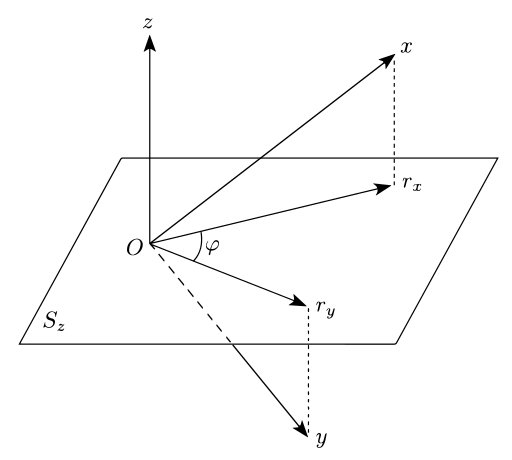
\includegraphics[width=\linewidth]{images/pcgeom.png}
\end{column}
\end{columns}
\bigskip

Ces deux points reviennent à regarder l'orthogonalité des projetés de Y et X sur le plan orthogonal à Z.
\end{frame}

%====================================================================
\begin{frame}{Lien avec la matrice de précision}
\bleu{Gaussien :} Soit   $X\sim \mathcal{N}(\mu, \Omegab^{-1})$ et la régression
$X_j = \sum_{k\neq j} \beta_{jk} X_k + \varepsilon_j$. Alors $\varepsilon_j \sim \Ncal (0, \omega_{jj}^{-1})$ et $ \beta_{jk} = -\omega_{jk}/\omega_{jj}.$
Donc $\emphase{\omega_{jk} \propto \beta_{jk}}$ 
\begin{center}
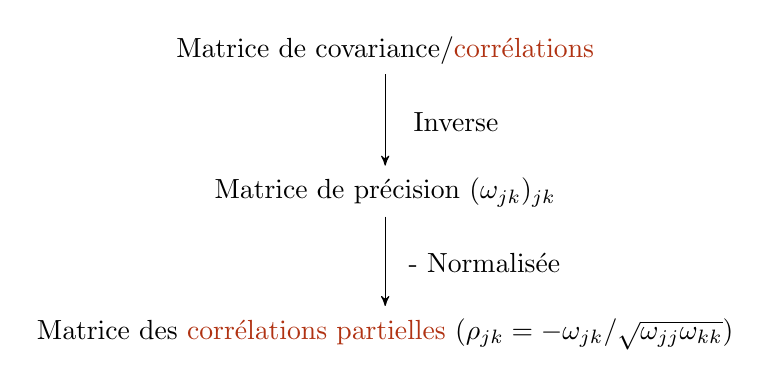
\begin{tikzpicture}	
      \tikzstyle{every edge}=[-,>=stealth',shorten >=1pt,auto,thin,draw]
		\node[] (A1) at (0,0) {Matrice de covariance/\emphase{corrélations}};
		\node[] (A2) at (0,-1*\length) {Matrice de précision $(\omega_{jk})_{jk}$};
		\node[] (A3) at (0,-2*\length) {Matrice des \emphase{corrélations partielles} ($\rho_{jk} =- \omega_{jk}/\sqrt{\omega_{jj} \omega_{kk}}$)};
		\node[] (A4) at (0.5*\length,-0.5*\length) {Inverse};
		\node[] (A5) at (0.7*\length,-1.5*\length) {- Normalisée};
		\path (A1) edge [->] (A2)
        (A2) edge [->] (A3);
\end{tikzpicture}  
\bigskip

 corrélation partielle/précision $\neq 0 \iff$ dépendance conditionnelle\\
  (en gaussien)\\
  \end{center}
\end{frame}
 %====================================================================
\begin{frame}{Dépendences conditionnelles entre espèces}
\textit{Mesure du lien de dépendance entre deux espèces $j$ et $k$, \emphase{après avoir contrôllé l'effet de toutes les autres}}.  \\
 \bigskip
 
  Ici c'est comme si on mesurait la corrélation entre les résidus des deux régressions des espèces $j$ et $k$  avec toutes les autres.\\
 \bigskip
 
  Inverser la matrice des corrélations :
\begin{itemize}
\item  permet d'obtenir toutes les mesures des dépendances conditionnelles en $\mathcal{O}(p^3)$ opérations,
\item améliore la précision des résultats en estimant jointement toutes les quantités,
\item passe moins à l'échelle que l'estimation par régressions (à étudier).
\end{itemize}
\end{frame}
 %====================================================================

\begin{frame}{Deux scénarios exemples}
\begin{columns}
\begin{column}{0.65\linewidth}
 
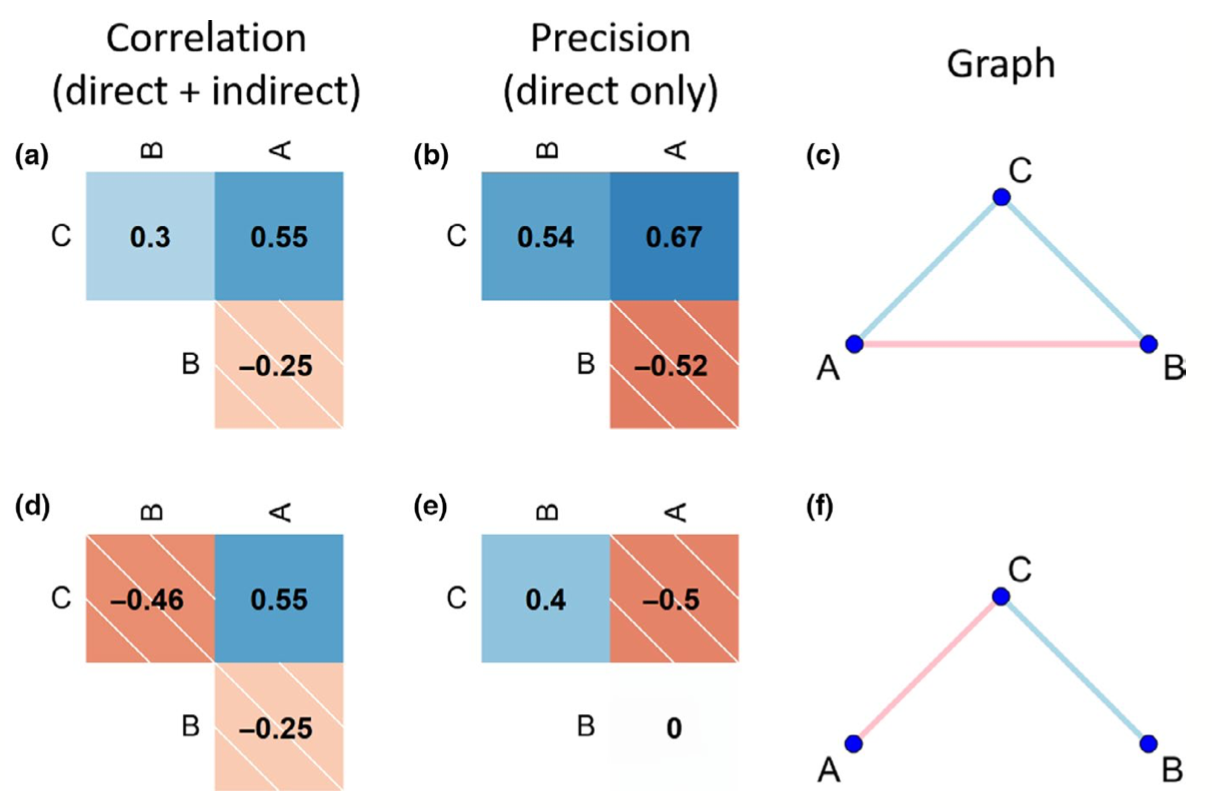
\includegraphics[width=\linewidth]{images/cor_parcor.png}
 
\end{column}
\begin{column}{0.35\linewidth}
\pause
\begin{itemize}
\item Même $Cor(A,B)$ pour les deux scénarios.
\item Les modèles graphiques gaussiens permettent d'étudier les dépendances conditionnelles.
\item Mais besoin de \emphase{passer en gaussien}.
\end{itemize}
\end{column}
\end{columns}
\end{frame}
 %====================================================================
\section{Modélisation}
\begin{frame}{Passage dans l'espace gaussien}
Plusieurs possibilités : transformation, variables latentes... Ici copules gaussiennes.
\bigskip

\bleu{Les copules gaussiennes} associent (couplent) une collection de distributions univariées avec une distribution gaussienne multivariée.
\bigskip

\begin{itemize}
\item Permettent d'\emphase{estimer une distirbution jointe} à partir de marginales
\item \emphase{Flexibles} sur la modélisation des marginales de départ : Poisson, Binomiale, Négative Binomiale, Multinomiale etc.
\item Le couplage se fait entre les fonctions de répartition marginales estimées (empiriquement ou avec un modèle paramétrique).
\end{itemize}
\end{frame}
 %====================================================================

\begin{frame}{Exemple jouet avec deux espèces}
\begin{columns}
\begin{column}{0.54\linewidth}
 
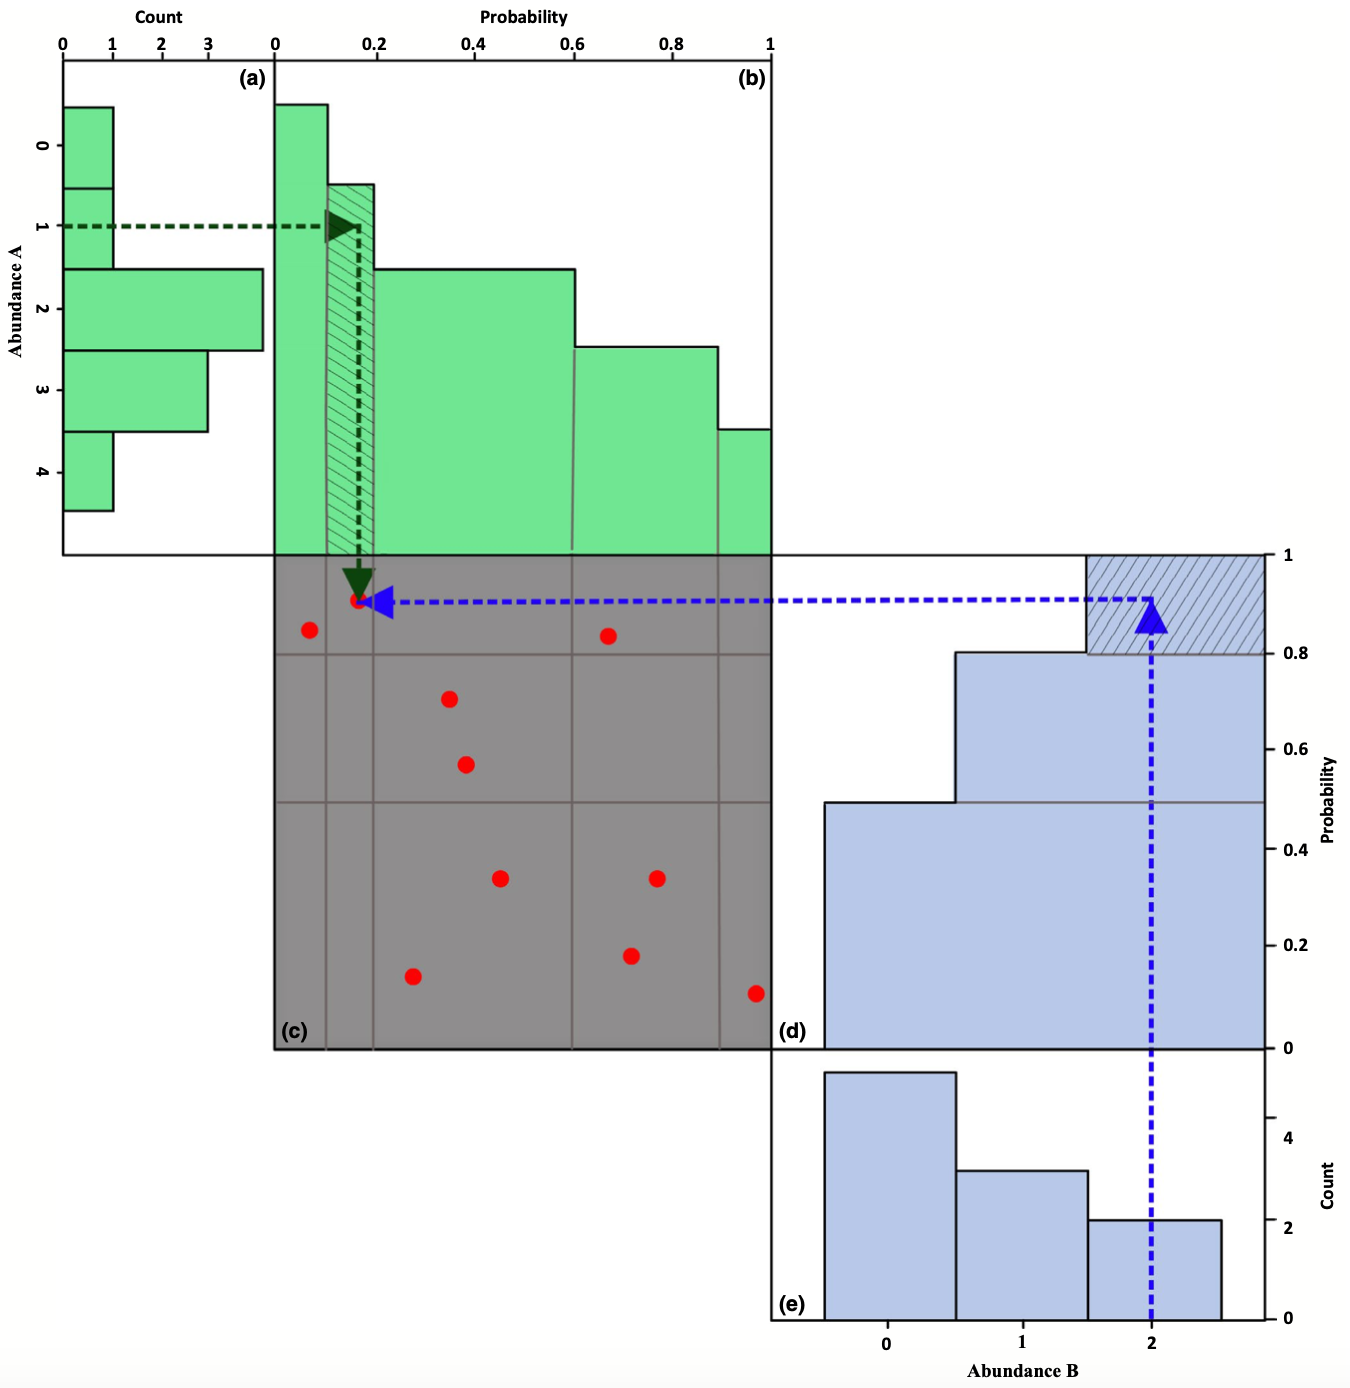
\includegraphics[height=7.3cm]{images/copula.png}
 
\end{column}
\begin{column}{0.45\linewidth}
\pause
\begin{enumerate}
\item Colonne : estimer de la fonction de répartition marginale de chaque espèce  sur l'ensemble des échantillons (b et d)\pause
\item Ligne : pour chaque échantillon, projeter l'abondance sur la région de répartition \pause
\item Obtenir un résidu par échantillon (c) en tirant uniformément dans cette région
\item Estimer les paramètres de la distribution jointe ($\rho_{AB}$)
\end{enumerate}
\end{column}
\end{columns}
\end{frame}

%====================================================================
\begin{frame}{Gaussian copula graphical models}
Package \texttt{ecoCopula} sur le CRAN :\\
\bigskip

\begin{enumerate}
\item Ajuste les covariables par un modèle linéaire généralisé multivarié (\texttt{mvabund::manyglm()})
\item Estime une matrice de covariance des résidus (en fait plusieurs fois, pour estimer la loi des résidus)
\item Infère le graph avec \texttt{glasso}
\end{enumerate}
\end{frame}
%====================================================================
\begin{frame}{glasso}

  Soit $\Ybf\sim \mathcal{N}(\mu, \Omegab^{-1})$. Alors :
\vspace{0.3cm}
\begin{columns}
\begin{column}{0.4\linewidth}
  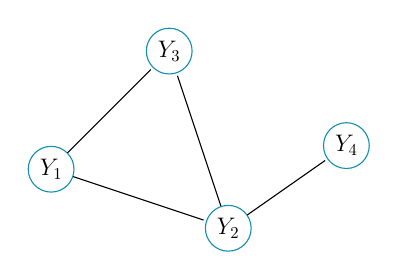
\begin{tikzpicture}
      \tikzstyle{every edge}=[-,>=stealth',shorten >=1pt,auto,thin,draw]
		\node[observed] (A1) at (0*\edgeunit, 0*\edgeunit) {$Y_1$};
	\node[observed] (A2) at (1.5*\edgeunit, -0.5*\edgeunit) {$Y_2$};
		\node[observed] (A3) at (1*\edgeunit, 1*\edgeunit) {$Y_3$};
		\node[observed] (A4) at (2.5*\edgeunit, 0.2*\edgeunit) {$Y_4$};
		\path (A1) edge [] (A2)
        (A1) edge [] (A3)
        (A2) edge [] (A3)
        (A2) edge [] (A4);
       % (A1) edge[Complement,dashed] (A4)
        %(A3) edge[Complement,dashed] (A4);
\end{tikzpicture}
\end{column}
\begin{column}{0.1\linewidth}
\emphase{$\iff$ }
\end{column}
\begin{column}{0.4\linewidth}
$\Omegab=\left(\begin{array}{llll}
*&*&*&\emphase{0}\\
*&*&*&*\\
*&*&*&\emphase{0}\\
\emphase{0}&*&\emphase{0}&*
\end{array}\right) $
\end{column}
\end{columns}
\bigskip

Le Graphical LASSO effectue une estimation par régularisation pénalisée
 $$\argmax_{\Omegab\geq 0} \big\{ \log |\Omegab| +tr{\Yb^\intercal \Yb \Omegab}- \lambda ||\Omegab||_1\big\}, \qquad ||\Omegab||_1 = \sum_{j\neq k} |\omega_{jk}|.$$
 
 La pénalité $\ell-1$ sur $\Omegab$ permet d'obtenir des vrais $0$.
\end{frame}
\section{Resultats}
\begin{frame}{Simulations}
\begin{figure}
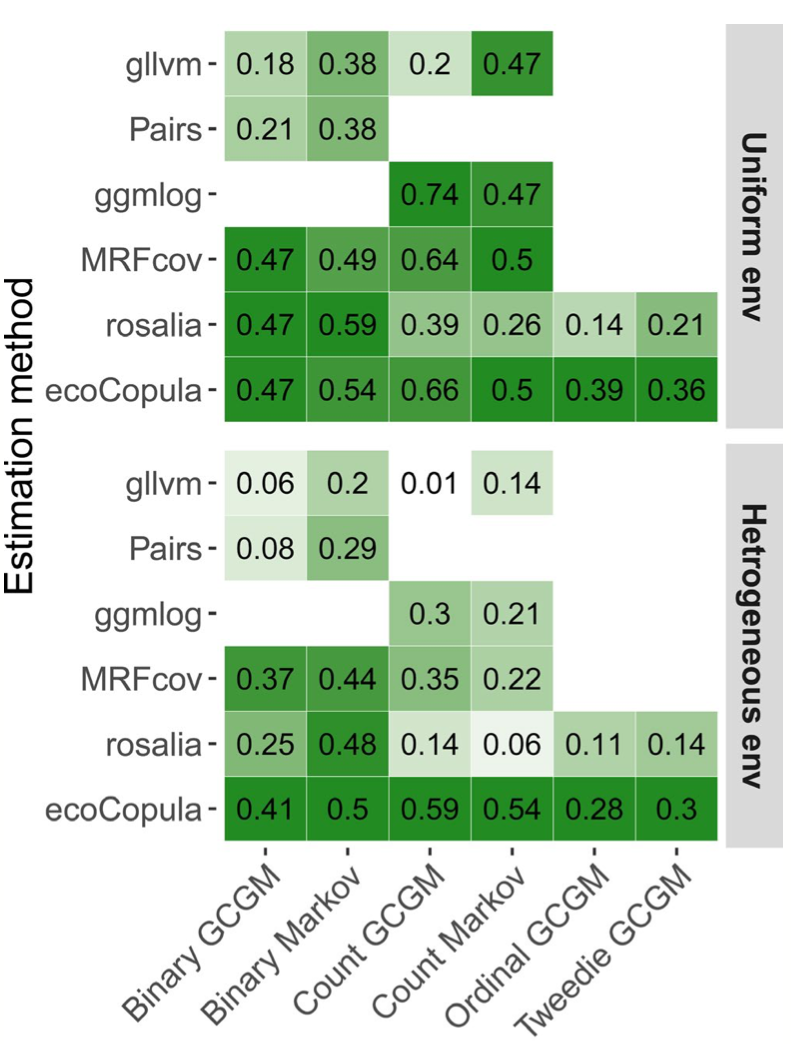
\includegraphics[height=7cm]{images/simu.png}
\end{figure}
\end{frame}
\begin{frame}{Analyse de données: Spiders dataset}
\begin{figure}
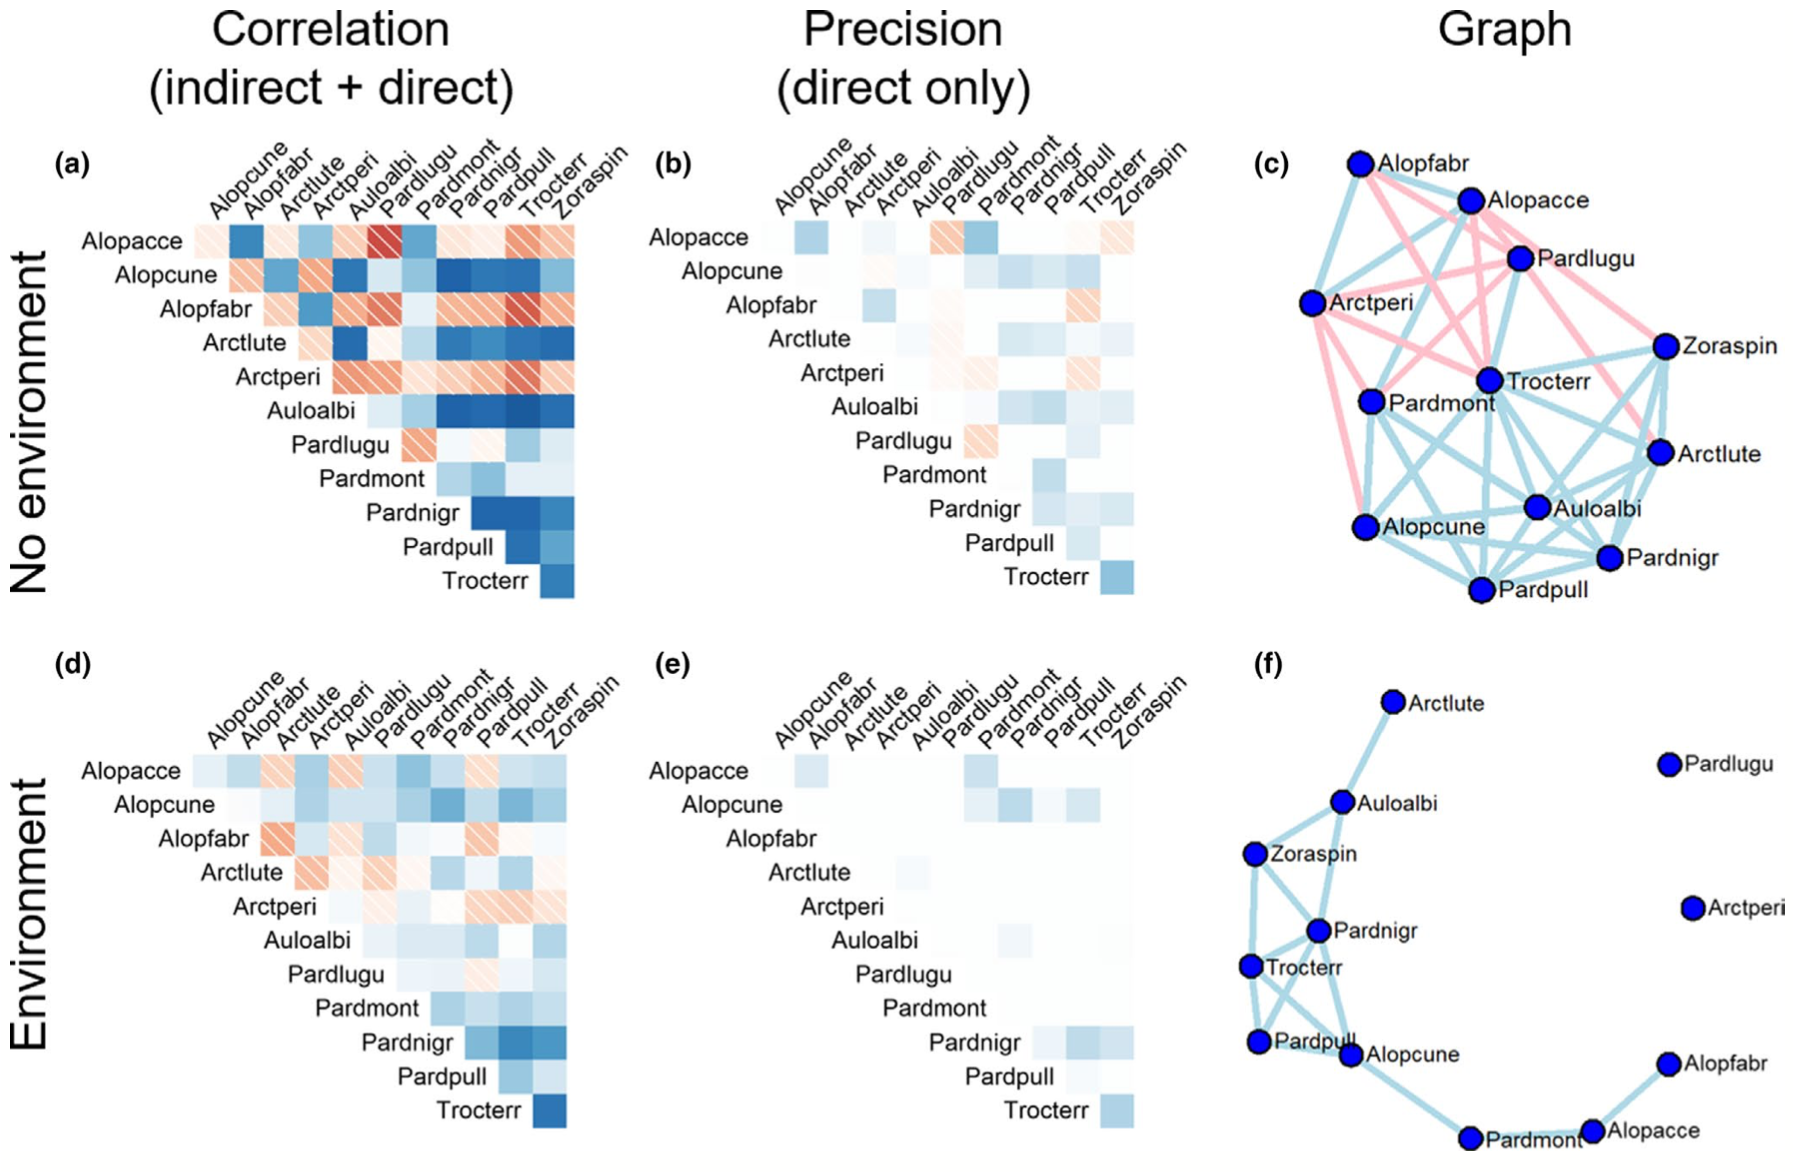
\includegraphics[height=7cm]{images/ex1.png}
\end{figure}
\end{frame}
\begin{frame}{Conclusion}
\begin{itemize}
\item Une méthode efficace pour l'inférence de réseaux de dépendances conditionnelles
\item Flexibilité sur les données en entrée
\item Flexibilité sur la modélisation des covariables
\item Permet de traiter de gros jeux de données (ex : 900x1300)
\end{itemize}

\end{frame}
\end{document}